\documentclass[titlepage]{scrartcl}
\usepackage{enumitem}
\usepackage[british]{babel}
\usepackage[style=apa, backend=biber]{biblatex}
\DeclareLanguageMapping{british}{british-apa}
\usepackage{url}
\usepackage{float}
\usepackage{caption}
\restylefloat{table}
\usepackage{perpage}
\MakePerPage{footnote}
\usepackage{abstract}
\usepackage{graphicx}
% Create hyperlinks in bibliography
\usepackage{hyperref}
\usepackage{amsmath}

\usepackage[T1]{fontenc}
\usepackage[utf8]{inputenc}
\usepackage{blindtext}
\setkomafont{disposition}{\normalfont\bfseries}

\graphicspath{
    {./resources/},
}
\addbibresource{~/Documents/library.bib}


\newsavebox{\abstractbox}
\renewenvironment{abstract}
  {\begin{lrbox}{0}\begin{minipage}{\textwidth}
   \begin{center}\normalfont\sectfont\abstractname\end{center}\quotation}
  {\endquotation\end{minipage}\end{lrbox}%
   \global\setbox\abstractbox=\box0 }

\usepackage{etoolbox}
\makeatletter
\expandafter\patchcmd\csname\string\maketitle\endcsname
  {\vskip\z@\@plus3fill}
  {\vskip\z@\@plus2fill\box\abstractbox\vskip\z@\@plus1fill}
  {}{}
\makeatother

\DeclareCiteCommand{\citeyearpar}
    {}
    {\mkbibparens{\bibhyperref{\printdate}}}
    {\multicitedelim}
    {}

% MATLAB Code block stuff...
\usepackage{color}
\usepackage{listings}

\definecolor{dkgreen}{rgb}{0,0.6,0}
\definecolor{gray}{rgb}{0.5,0.5,0.5}

\newcommand{\code}[1]{\texttt{#1}}

\lstset{language=Matlab,
    keywords={break,case,catch,continue,else,elseif,end,for,function,
        global,if,otherwise,persistent,return,switch,try,while},
    basicstyle=\ttfamily,
    keywordstyle=\color{blue},
    commentstyle=\color{gray},
    stringstyle=\color{dkgreen},
    numbers=left,
    numberstyle=\tiny\color{gray},
    stepnumber=1,
    numbersep=10pt,
    backgroundcolor=\color{white},
    tabsize=4,
    showspaces=false,
    showstringspaces=false
    frame=single,
    breaklines=true,
    %postbreak=\raisebox{0ex}[0ex][0ex]{\ensuremath{\color{red}\hookrightarrow\space}}
}

\begin{document}
\title{ECS708P/U - Machine Learning}
\subtitle{\LARGE{Assignment 1 Report\\Linear and Logistic Regression}}
\author{Sam Perry - EC16039}

\maketitle

\section{Linear Regression}
\subsection{Modify the function \code{calculate\_hypothesis.m} to return the predicted value for a single specified training example}
\begin{lstlisting}
function hypothesis = calculate_hypothesis(X, theta, training_example)
    % Calculates the hypothesis for a given X, theta and specified training example
    % Get bias term
    x0 = X(training_example, 1);
    % Get first term
    x1 = X(training_example, 2);

    % Calculate output hypothesis
    hypothesis = theta(1)*x0+theta(2)*x1;
end
\end{lstlisting}

\subsection{Notice that the hypothesis function is not being used in the
\code{gradient\_descent} function. Modify this to use the
\code{calculate\_hypothesis} function}
\begin{lstlisting}
function theta = gradient_descent(X, y, theta, alpha, iterations, do_plot)
    %GRADIENT_DESCENT do Gradient Descent for a given X, y, theta, alpha
    %for a specified number of iterations

    %if less than 6 arguments was given, then set do_plot to be false
    if nargin < 6
        do_plot = false;
    end
    if(do_plot)
        plot_hypothesis(X, y, theta);
        drawnow; pause(0.1); 
    end

    m = size(X, 1); %number of training examples
    cost_vector = []; %will store the results of our cost function

    for it = 1:iterations
        %%%%%%%%%%%%%%%%%%%
        % gradient descent
        %%%%%%%%%%%%%%%%%%%

        theta_0 = theta(1);
        theta_1 = theta(2);

        %update theta(1) and store in temporary variable theta_0
        sigma = 0.0;

        for i = 1:m
            hypothesis = calculate_hypothesis(X, theta, i);
            output = y(i);
            sigma = sigma + (hypothesis - output);
        end

        theta_0 = theta_0 - ((alpha * 1.0) / m) * sigma;


        %update theta(2) and store in temporary variable theta_1
        sigma = 0.0;

        for i = 1:m
            hypothesis = calculate_hypothesis(X, theta, i);
            output = y(i);
            sigma = sigma + (hypothesis - output) * X(i, 2);
        end

        theta_1 = theta_1 - ((alpha * 1.0) / m) * sigma;

        %update theta
        theta = [theta_0, theta_1];

        %update cost_vector
        cost_vector = [cost_vector; compute_cost(X, y, theta)];

        if do_plot
            plot_hypothesis(X, y, theta);
            drawnow; pause(0.1); 
        end
    end

    disp 'Gradient descent is finished.'
        
    if do_plot
        disp 'Press enter!'
        pause;
    end

    plot_cost(cost_vector);
        
    disp 'Press enter!';
    pause;
end
\end{lstlisting}
 
\subsection{Observe what happens when you use a very high or very low learning
rate}
When a very low alpha value ($\alpha=0.0001$) is used, the reduction in cost per
iteration is not sufficient to generate an accurate function. This is
illustrated in figures~\ref{LowLearnFunc} and ~\ref{LowLearnCost}

\begin{figure}[H]
    \caption{Hypothesis Function ($\alpha=0.0001$)}
    \makebox[\textwidth]{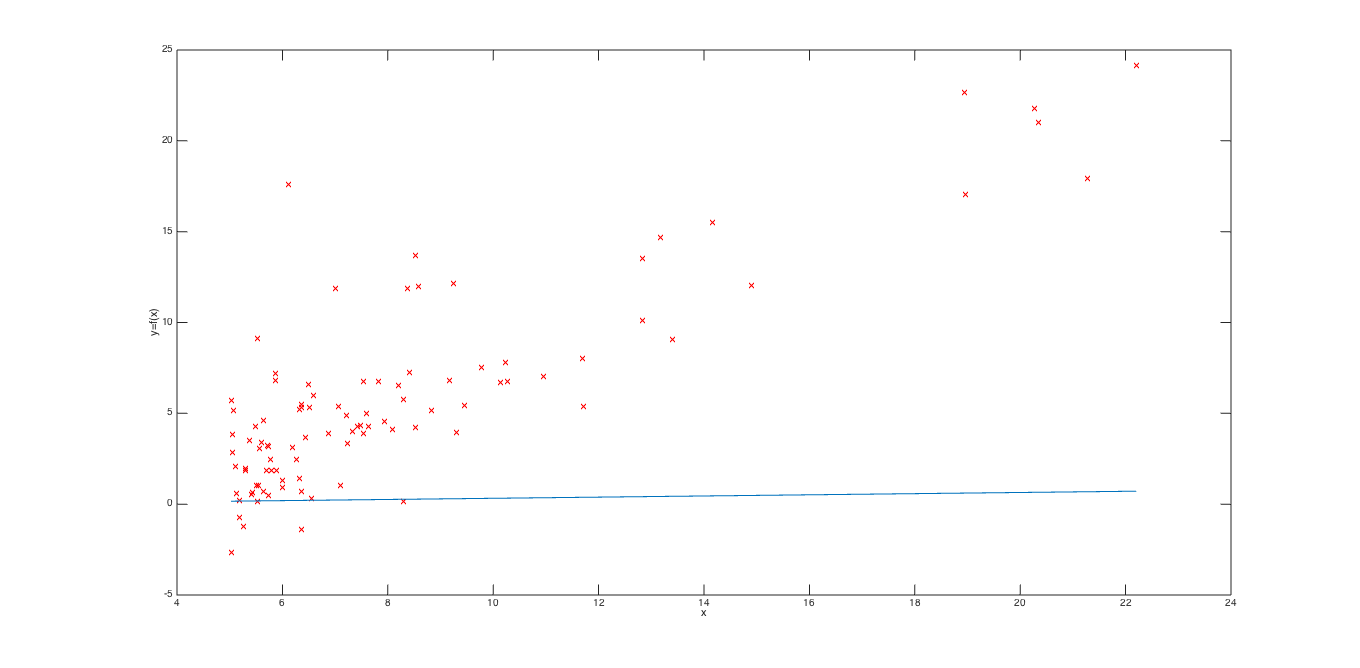
\includegraphics[width=1\textwidth]{LowLearningRateFunc}}
    \label{LowLearnFunc}
    \caption{Cost Function ($\alpha=0.0001$)}
    \makebox[\textwidth]{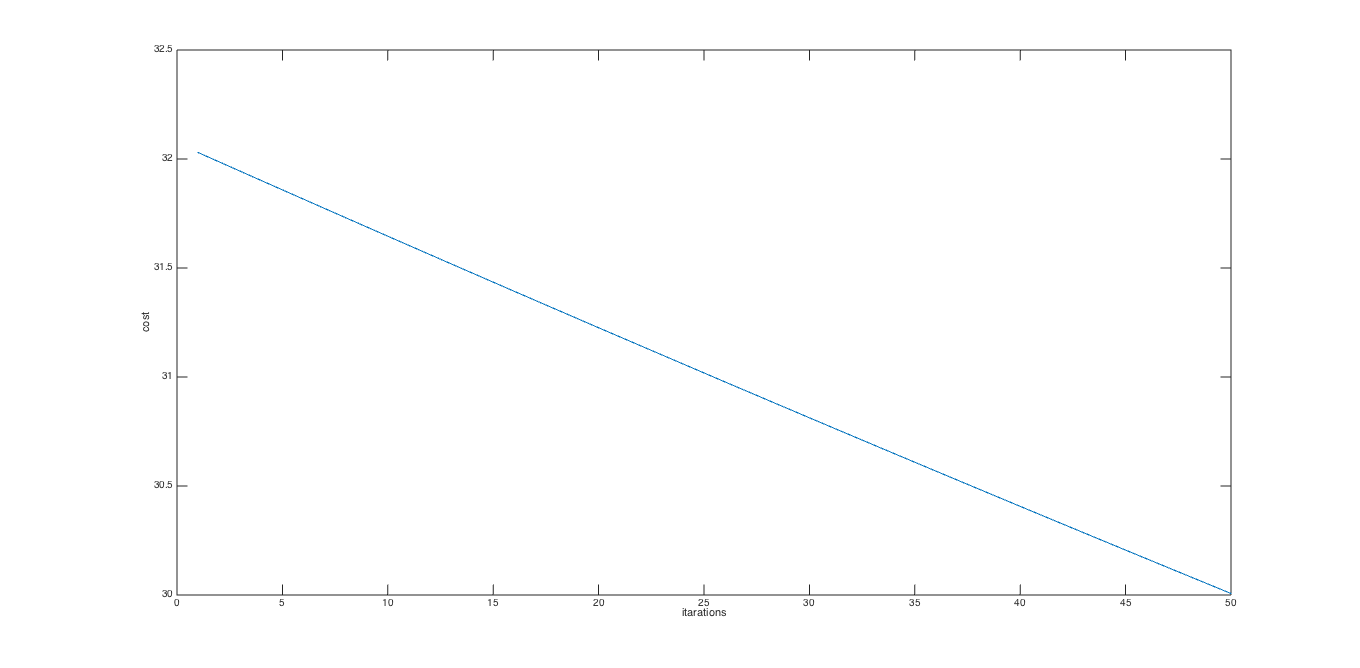
\includegraphics[width=1\textwidth]{LowLearningRateCost}}
    \label{LowLearnCost}
\end{figure}

A high value for alpha ($\alpha=1.0$) will result in large shifts in the
function over each iteration. This causes the function to shift between
positive and negative at ever increasing cost on each iteration. The final
result of this can be seen in figure~\ref{HighLearnFunc}. The exponential
increase in cost causes only the final increase to be clear through
figure~\ref{HighLearnCost}.

\begin{figure}[H]
    \caption{Hypothesis Function ($\alpha=1.0$)}
    \makebox[\textwidth]{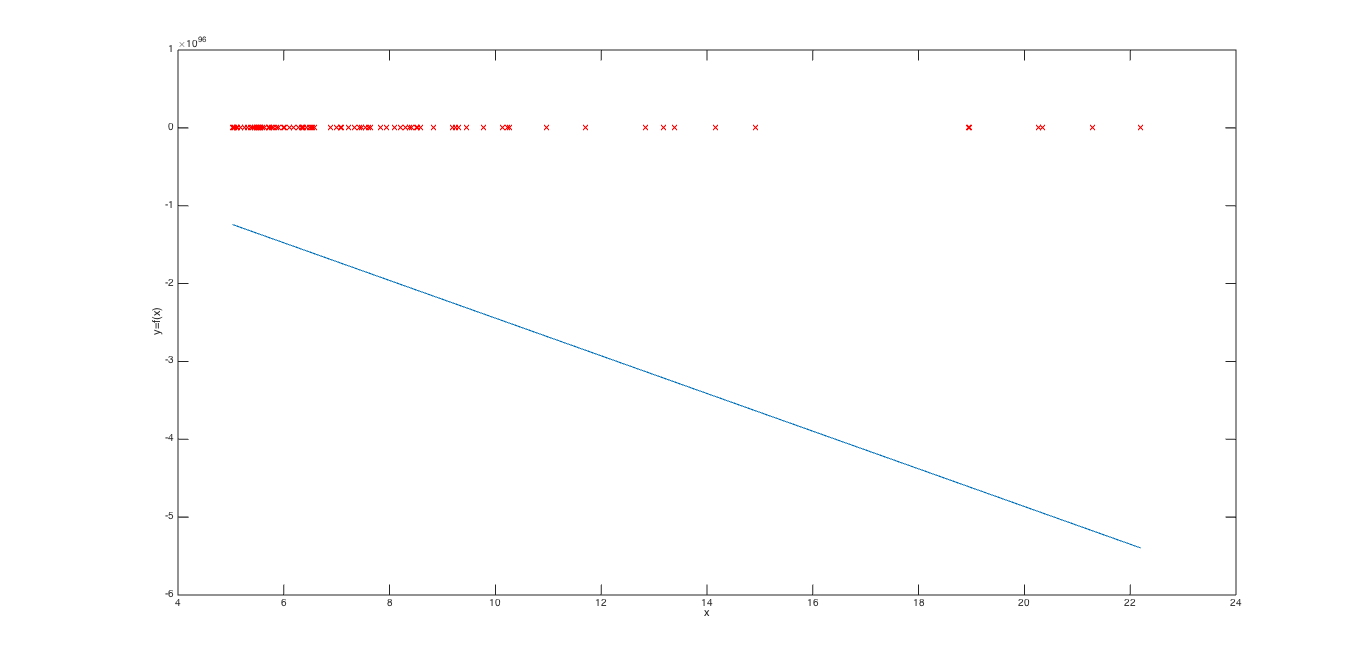
\includegraphics[width=1\textwidth]{HighLearningRateFunc}}
    \label{HighLearnFunc}
    \caption{Cost Function ($\alpha=1.0$)}
    \makebox[\textwidth]{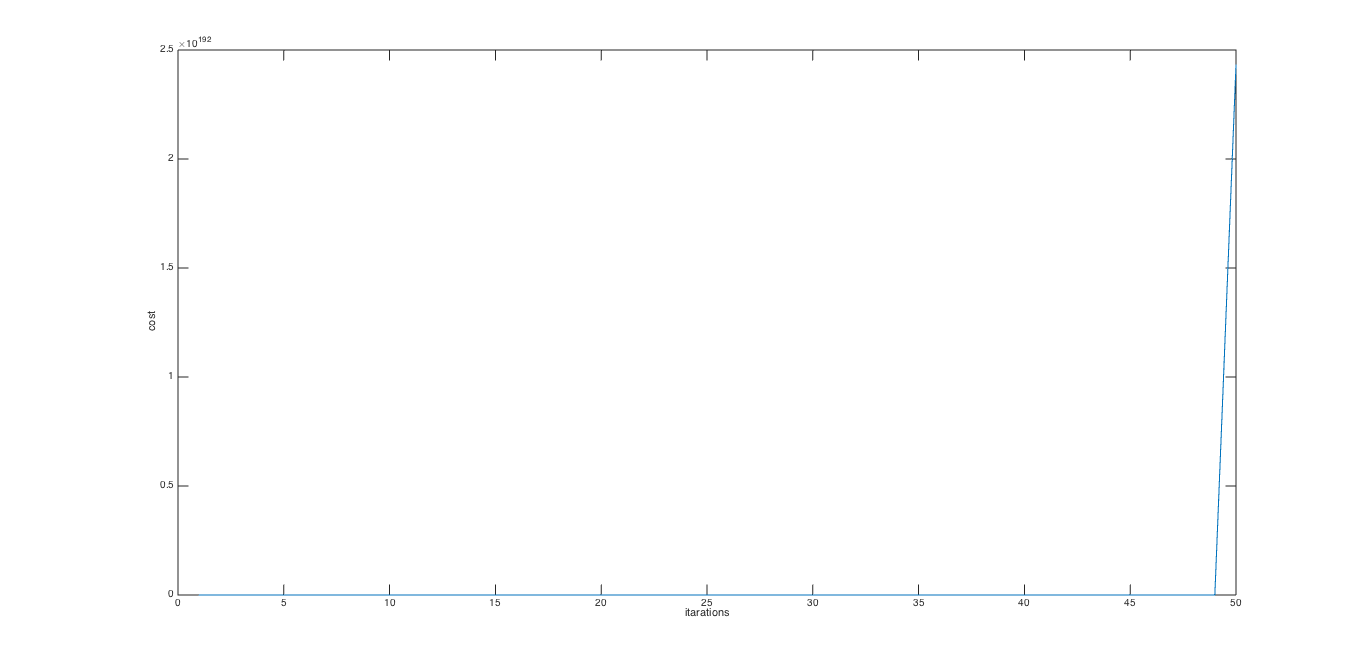
\includegraphics[width=1\textwidth]{HighLearningRateCost}}
    \label{HighLearnCost}
\end{figure}

% \printbibliography
\end{document}
